\documentclass[11pt, ngerman]{beamer}
\usetheme{Goettingen}
\usecolortheme{seahorse}
\setbeamertemplate{footline}[frame number]
\usepackage{graphicx}
\usepackage{subfigure}
\usepackage{amsmath}
\author{Marie-Sophie Briem, Inga Lemme, Sarah Weber}
\title{\textrm \textbf{Ein systematischer Vergleich von Verfahren zur funktionellen und
taxonomischen Klassifikation von metagenomischen Sequenzfragmenten}}
\setbeamercovered{transparent} 
\setbeamertemplate{navigation symbols}{} 
\date{29.01.2016}
\institute{Zentrum f\"ur Bioinformatik, Universit\"at Hamburg} 

\begin{document}

\begin{frame} %Title
\setbeamercovered{transparent}
\titlepage
\end{frame}


\begin{frame} %Gliederung
\frametitle{Gliederung}
\tableofcontents 
\end{frame} 
 

\section{Motivation} 
\begin{frame} %Motivation
\frametitle{Motivation}
\begin{itemize}
\item Lambda und Diamond: Programme zur funktionelle und taxonimischen Klassifizierung von metagenomischen Sequenzfragmenten
\item Was ist Metagenome? 
\item Problemstellung: Systematischer Vergleiche von Lambda und Diamond
\end{itemize}
\end{frame}

\section{Projekt-Plan}
\begin{frame}
\frametitle{Projekt-Plan}
\begin{enumerate}
\item Datens\"atze mit Lambda und Diamond gegen eine Datenbank alignieren
  \begin{itemize}
    \item Ausgabe enth\"alt Readnr, Gi/Refseq-Nr
  \end{itemize}
\item Lambda- und Diamondoutput mithilfe von Megan mappen
  \begin{itemize}
    \item Ausgabe enth\"alt Readnr, Taxid
  \end{itemize}
\item Goldstandart aller Datens\"atze erstellen
  \begin{itemize}
    \item Enth\"alt Readnr, Taxid, Gi/Refseq-Nr
  \end{itemize}
\item Taxids von Meganoutput und Goldstadart vergleichen (Taxtree)
  \begin{itemize}
    \item Ausgabe: Distanzen zweier Taxid im Taxtree
  \end{itemize}
\end{enumerate}
\end{frame}

\section{Methoden}
\subsection{Vorarbeit}
\begin{frame} %Vorarbeit
\frametitle{Vorarbeit}
\begin{itemize}
\item Datens\"atze und Datenbanken downloaden
\begin{itemize}
  \item Folgende Datens\"atze: Carma, Facs, Metaphyler, Phylopythia, PhymmBL und Raiphy
  \item Problem: einige Datens\"atze nicht vollst\"andig verf\"ugbar
  \item Lambda Datenbank indexen
\end{itemize}
\item Programme Lambda und Diamond downloaden
\end{itemize}
\end{frame}

\subsection{Parser}
\begin{frame}
\frametitle{Parser}
\begin{itemize}
\item Parser beschreiben
\item Probleme
\end{itemize}
\end{frame}
\section{Ergebnisse}
\begin{frame}
\frametitle{Lambda}
\begin{figure}
    \noindent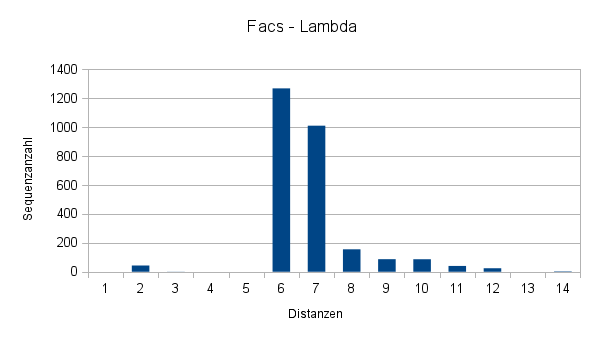
\includegraphics[width=\linewidth,height=7cm,
keepaspectratio]{facs_verteilung.png}
\end{figure}
\end{frame}

\begin{frame}
\frametitle{Diamond}
\end{frame}
\section{Fazit und Ausblick}
\begin{frame}
\frametitle{Fazit}
\begin{itemize}
\item
\end{itemize}
\end{frame}

\begin{frame}
\frametitle{Ausblick}
\begin{itemize}
\item
\end{itemize}
\end{frame}


\end{document}
